\section{二分图与匹配}
\label{sec:04-Discrete-Mathematics/03-Graph-Theory/04}

内容审核团队今天有 11 名在岗的审核员和 9 条按语种划分的待处理队列。每个人只认得其中几种语言，每条队列同一时刻只安排一个人盯，每个人也只盯一条。目标很朴素：让尽可能多的队列有人守着。

先按名单顺序派：轮到谁，就把他能做的、还空着的队列里随便给一条。派到最后卡住了，还剩两条队列没人。问题出在第一步——某人只懂日语，日语队列却早被一个日语韩语都懂的人占去了，而那个人本可以去守韩语。贪心不会回头，它也不知道自己该回头。

要判断``还剩两条''是运气不好还是真的到顶，得先把问题从排班表里拆出来。

\subsection{边只在两组之间}

审核员一组，队列一组，``某人会某语种''连一条边。同组内部不连边——审核员之间不互相配对，队列之间也不。顶点集能这样劈成两半、所有边都跨组的图叫二分图。

哪些图是二分图？把顶点两染色，相邻的必须异色，能染成就是。这个说法等价于另一条更好用的判据：图里没有奇环。从任一顶点出发做广度优先搜索，按层的奇偶染色，同一层内部若出现一条边，这条边加上两个端点各自回到根的路径就凑出一个奇环；反过来，没有奇环，分层染色就不会出冲突。判定二分性因此只要一遍搜索，不必试遍所有染色方案。

奇环这个障碍在下一节还会再出现一次，那时它挡的是三色而不是两色。

\subsection{极大和最大差在哪}

匹配是一组两两不共端点的边：每个人至多接一条队列，每条队列至多派一个人。

贪心停下来的那个状态叫极大匹配——任何一条剩余的边都至少有一端被占了，再也塞不进去。最大匹配是边数最多的那个。两者的差距可以很大，前面那次派班就是例子。词只差一个字，含义是``局部加不动''与``全局最优''的区别，读文献时值得留神。

关键在于，卡住的时候有没有办法系统地退回去重排。

\begin{center}
\begin{tikzpicture}[x=1cm,y=1cm,font=\small,>=stealth]
  % 增广路高亮
  \draw[orange!70,line width=3pt,opacity=0.45] (0,3) -- (3.4,3) -- (0,2) -- (3.4,2) -- (0,1) -- (3.4,1);
  \draw[black!35] (0,3) -- (3.4,3);
  \draw[black!35] (0,2) -- (3.4,2);
  \draw[black!35] (0,1) -- (3.4,1);
  \draw[blue!75,line width=2pt] (0,2) -- (3.4,3);
  \draw[blue!75,line width=2pt] (0,1) -- (3.4,2);
  \draw[blue!75,line width=2pt] (0,0) -- (3.4,0);
  \foreach \y in {2,1,0}{\fill (0,\y) circle (2.6pt);}
  \foreach \y in {3,2,0}{\fill (3.4,\y) circle (2.6pt);}
  \draw[fill=white,black] (0,3) circle (2.6pt);
  \draw[fill=white,black] (3.4,1) circle (2.6pt);
  \node[left] at (-0.2,3) {\(\ell_1\)};
  \node[left] at (-0.2,2) {\(\ell_2\)};
  \node[left] at (-0.2,1) {\(\ell_3\)};
  \node[left] at (-0.2,0) {\(\ell_4\)};
  \node[right] at (3.6,3) {\(r_1\)};
  \node[right] at (3.6,2) {\(r_2\)};
  \node[right] at (3.6,1) {\(r_3\)};
  \node[right] at (3.6,0) {\(r_4\)};
  \node[black!70,font=\footnotesize] at (1.7,3.7) {翻转前：3 条匹配边};
  \begin{scope}[shift={(8.2,0)}]
    \draw[black!35] (0,2) -- (3.4,3);
    \draw[black!35] (0,1) -- (3.4,2);
    \draw[blue!75,line width=2pt] (0,3) -- (3.4,3);
    \draw[blue!75,line width=2pt] (0,2) -- (3.4,2);
    \draw[blue!75,line width=2pt] (0,1) -- (3.4,1);
    \draw[blue!75,line width=2pt] (0,0) -- (3.4,0);
    \foreach \y in {3,2,1,0}{\fill (0,\y) circle (2.6pt);\fill (3.4,\y) circle (2.6pt);}
    \node[left] at (-0.2,3) {\(\ell_1\)};
    \node[left] at (-0.2,2) {\(\ell_2\)};
    \node[left] at (-0.2,1) {\(\ell_3\)};
    \node[left] at (-0.2,0) {\(\ell_4\)};
    \node[right] at (3.6,3) {\(r_1\)};
    \node[right] at (3.6,2) {\(r_2\)};
    \node[right] at (3.6,1) {\(r_3\)};
    \node[right] at (3.6,0) {\(r_4\)};
    \node[black!70,font=\footnotesize] at (1.7,3.7) {翻转后：4 条匹配边};
  \end{scope}
\end{tikzpicture}

\emph{左边的蓝色匹配已经加不动了，可它不是最大的。空心点 \(\ell_1\) 与 \(r_3\) 都没被匹配，橙色那条路把它俩连起来，一路交替走非匹配边和匹配边。沿这条路把每条边的身份对调，路上原有的两条匹配边换成三条，其余顶点的匹配状态不变。}
\end{center}

这条路叫增广路：起点和终点都是未匹配顶点，中间的边非匹配与匹配交替出现。它的长度必然是奇数，两端各是一条非匹配边，所以翻转之后匹配边净增一条。中间的每个顶点翻转前后都恰好挂着一条匹配边，只是换了一条，不会有人同时接两条。

Berge 定理把这条观察反过来用：一个匹配是最大的，当且仅当不存在增广路。必要性就是上面这段。充分性的骨架是取当前匹配 \(M\) 与任一更大匹配 \(M'\) 的对称差，这个子图里每个顶点最多挂两条边（一条来自 \(M\)，一条来自 \(M'\)），因此它只由路径和偶环组成；\(M'\) 更大，就必有一段 \(M'\) 的边比 \(M\) 多，那一段只能是一条相对 \(M\) 的增广路。

它的价值在于把``是不是全局最优''换成了``能不能找到一条路''。前者要跟所有匹配比，后者一次搜索就有答案。匈牙利算法、Hopcroft--Karp 都在做同一件事，区别只是每轮找几条增广路。

\subsection{配不上的时候，是哪一撮卡住了}

把目标提高一点：不满足于最大，而要求左侧每个顶点都配上（左完美匹配）。什么时候办得到？

有一个显然的必要条件。取左侧任意一撮顶点 \(S\)，它们的邻居合起来记作 \(N(S)\)。这撮人只能在 \(N(S)\) 里面找位置，位置不够就一定有人落空。所以必须

\[
\abs{N(S)}\ge\abs{S},\qquad \text{对每个 }S\subseteq L.
\]

Hall 定理说这个条件也是充分的。分量不轻——它意味着失败必定留下证据，而且证据是局部的。

\begin{center}
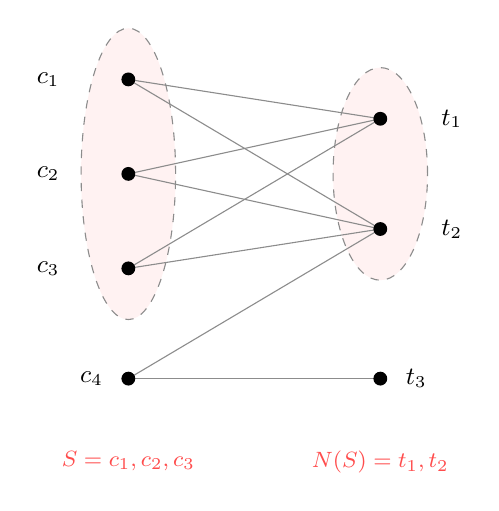
\begin{tikzpicture}[x=1cm,y=1cm,font=\small,>=stealth]
  \draw[black!45,dashed,fill=red!5] (0,1.2) ellipse (0.6 and 1.85);
  \draw[black!45,dashed,fill=red!5] (3.2,1.2) ellipse (0.6 and 1.35);
  \foreach \y in {2.4,1.2,0}{
    \draw[black!45] (0,\y) -- (3.2,1.9);
    \draw[black!45] (0,\y) -- (3.2,0.5);}
  \draw[black!45] (0,-1.4) -- (3.2,0.5);
  \draw[black!45] (0,-1.4) -- (3.2,-1.4);
  \foreach \y in {2.4,1.2,0,-1.4}{\fill (0,\y) circle (2.5pt);}
  \foreach \y in {1.9,0.5,-1.4}{\fill (3.2,\y) circle (2.5pt);}
  \node[left] at (-0.75,2.4) {\(c_1\)};
  \node[left] at (-0.75,1.2) {\(c_2\)};
  \node[left] at (-0.75,0) {\(c_3\)};
  \node[left] at (-0.2,-1.4) {\(c_4\)};
  \node[right] at (3.85,1.9) {\(t_1\)};
  \node[right] at (3.85,0.5) {\(t_2\)};
  \node[right] at (3.4,-1.4) {\(t_3\)};
  \node[below,red!70,font=\footnotesize] at (0,-2.2) {\(S=\set{c_1,c_2,c_3}\)};
  \node[below,red!70,font=\footnotesize] at (3.2,-2.2) {\(N(S)=\set{t_1,t_2}\)};
\end{tikzpicture}

\emph{三门课要各配一位不同的授课教师，可这三门课能胜任的老师全都只落在两个人身上。教师池整体可以很大，\(t_3\) 也闲着，但他一门都教不了。\(\abs{N(S)}=2<3=\abs{S}\)，排课在这一撮上必定失败。}
\end{center}

图里的信息量在于它指出该改什么。总量核对（老师比课多）通不过这一关；要解开死结，只能扩充这三门课的候选教师，或者砍掉其中一门。Hall 定理证明的构造性一面正好给出这撮 \(S\)：当最大匹配漏掉了左侧某个顶点，从它出发沿``非匹配边去右、匹配边回左''走遍所有可达顶点，走到的那批左顶点就是违反条件的 \(S\)。定理与诊断工具是一回事。

\subsection{最大与最小对上了}

在二分图上还有一条更利落的等式。顶点覆盖是一组顶点，使得每条边至少有一端在里面。König 定理断言：二分图的最大匹配数等于最小顶点覆盖数。

两边的方向是相反的。匹配是从下往上顶——每找到一条互不冲突的边，就说明答案至少这么大；覆盖是从上往下压——每给出一组能盖住所有边的顶点，就说明匹配不可能超过这个数（匹配的每条边都得被盖到，而一个覆盖顶点最多盖住其中一条）。所以任何一个匹配的大小不超过任何一个覆盖的大小，这一半是白送的。定理说的是两者能顶到一起。

这种``最大等于最小''的格局在\hyperref[sec:04-Discrete-Mathematics/03-Graph-Theory/02]{``路径、环与连通性''}里已经露过一面（Menger 定理），在网络流里叫最大流最小割，在连续优化里就是强对偶。事实上二分匹配可以写成一个线性规划，它的对偶恰好是顶点覆盖，而这个规划的约束矩阵有一种特殊结构，保证最优解落在整点上——这正是组合问题与\hyperref[sec:09-Convex-Optimization/05-Duality/02]{``对偶间隙何时闭合''}讨论的间隙闭合条件在同一处相遇。König 定理是那套理论最早、也最容易画出来的样本。

边带权重时，问题变成指派问题：不是配得多，而是配得好。目标换成总权最大，增广路的思路仍然管用，只是每次要沿着``能提升总权''的交替路走。推荐系统里的一轮分发、广告位与广告主的撮合、调度器把任务放到机器上，模型层面都是这一类，区别只在权重怎么算。

\subsection{它没管偏好，也没管冲突}

最大匹配假设有一个中央规划者，他要的是总量或总权。这里面没有参与者的意愿——审核员想不想守那条队列，模型不问。也没有任何一组顶点``不能同时选''的约束——二分图的两侧本身就把冲突关系限死了。

这两个缺口各自通向一节。偏好那条留到本章后面的\hyperref[sec:04-Discrete-Mathematics/03-Graph-Theory/06]{``稳定匹配与延迟接受''}。冲突那条更近：把``某两个东西不能共用一份资源''直接画成边，问题就变成给顶点分配资源标签，相邻的不许相同。二分图不过是这个问题恰好用两个标签就够的特例。下一节把标签数放开。
